\documentclass[lettersize,journal]{IEEEtran} % package ieeetran, tlmgr install ieeetran avec TexLive
\usepackage{amsmath,amsfonts}
\usepackage{algorithmic}
\usepackage{algorithm} % package algorithms
\usepackage{array}
\usepackage[caption=false,font=normalsize,labelfont=sf,textfont=sf]{subfig} % package subfig
% On a aussi besoin du package caption
\usepackage{textcomp}
\usepackage{stfloats} % package sttools
\usepackage{url}
\usepackage{verbatim}
\usepackage{graphicx}
\usepackage{tikz}
\usepackage{cite}
% Aussi besoin de la font pcrr7t qui est dans le package courier
\hyphenation{op-tical net-works semi-conduc-tor IEEE-Xplore}
% updated with editorial comments 8/9/2021

\begin{document}

\title{Comparison of different routing algorithms for Public Switched Telephone Networks (PSTN)}

\author{IEEE Publication Technology,~\IEEEmembership{\textsc{Fraty} Quentin, \textsc{Barniaudy} Maxime, \textsc{Maillet} Nathan,~IEEE,}
        % <-this % stops a space
\thanks{This paper was produced by the ENSEEIHT ASR Students.}% <-this % stops a space
\thanks{Manuscript received January 20, 2023; revised January 21, 2023.}}

% The paper headers
\markboth{N7's Journal of Network Architectures,~Vol.~1, No.~1, January~2023}%
{Shell \MakeLowercase{\textit{et al.}}: A Sample Article Using IEEEtran.cls for IEEE Journals}

%\IEEEpubid{0000--0000/00\$00.00~\copyright~2023 IEEE}
% Remember, if you use this you must call \IEEEpubidadjcol in the second
% column for its text to clear the IEEEpubid mark.

\maketitle

\begin{abstract}
        Public Switched Telephone Networks (or PSTN for short) heavily rely on a complex
        routing algorithm used to route calls between users. A good routing algorithm can
        support higher network loads, and limit the damage caused to users in case of a network
        breakdown. This study will show the different benefits and drawbacks of several routing algorithms,
        namely MTP-3 routing, load balancing routing, and adaptative routing. We also implemented a Dijkstra's 
        shortest path-based algorithm whose performance will be compared to the others.
\end{abstract}

\begin{IEEEkeywords}
Network, PSTN, Telephone, Routing algorithms, IEEE
\end{IEEEkeywords}

\section{Introduction}
\IEEEPARstart{T}{he} goal of this project was to compare
the efficiency of different routing methods, under different load conditions, and in case of a switch / link failure.

\section{Answer to questions \& State of the art}
\subsection{semaphore network of considered topology}

        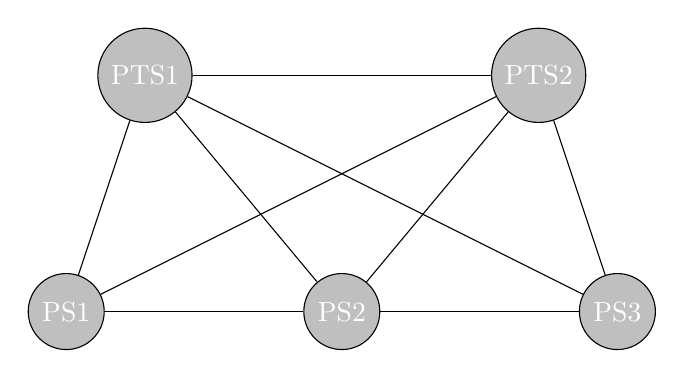
\begin{tikzpicture}
                \node[circle,draw,text=white,fill=lightgray] (PTS1) at (1,3){PTS1};
                \node[circle,draw,text=white,fill=lightgray] (PTS2) at (6,3){PTS2};
                \node[circle,draw,text=white,fill=lightgray] (PS1) at (0,0){PS1};
                \node[circle,draw,text=white,fill=lightgray] (PS2) at (3.5,0){PS2};
                \node[circle,draw,text=white,fill=lightgray] (PS3) at (7,0){PS3};

                \draw[-] (PTS1) -- (PTS2);
                \draw[-] (PTS1) -- (PS1);
                \draw[-] (PTS1) -- (PS2);
                \draw[-] (PTS1) -- (PS3);
                \draw[-] (PTS2) -- (PS1);
                \draw[-] (PTS2) -- (PS2);
                \draw[-] (PTS2) -- (PS3);
                \draw[-] (PS1) -- (PS2);
                \draw[-] (PS2) -- (PS3);
        \end{tikzpicture}

\subsection{Information needed to route with load balancing}
A load balancing routing protocol is defined by the fact that the routing decision is
only affected by the capacity of the different wires connected to the current node. Hence, 
in order to implement such algorithm, one needs to know beforehand the total capacity of the
different wires of his architecture. In real life, such algorithm is very easy to set up,
as a PSTN operator has the full knowledge of the network.

In the network proposed as an example in the subject, and for a communication between CA1 and CA3,
a load-balancing protocol would make the following decisions:
\begin{itemize}
        \item On the CA1 node, three links are available to be used by the routing algorithm.
        Supposedly, let's pretend that CA-CTS links have twice the capacity of CA-CA links.
        In that context, 40\% of the traffic would be directed to each CTS and the remaining 20\% 
        would be routed to CA2.
        \item In a load balancing algorithm, and without any other customization, there could be 
        some kind of loop. For example, in the CTS1 node, the load balancing algorithm could be
        forwarding messages coming from CA1 towards CA1! To prevent that problem, a geographical
        adressing can be put in place for the different nodes / clients. With that parameter taken
        into consideration during the load balancing algorithm, CTS1 would only have three possible
        links that get the current packet closer to the destination (CA1 - CTS1 being omitted).\\
        With the same capacity assumption as before, the load balancing algorithm would then route
        50\% of the communications from CA1 to CA3 through CTS2, and 25\% to CA2 and CA3.       
\end{itemize} 

% Risque
The main risk with such routing is that if the main link breaks, we will route most of the
traffic there while our data will be lost. The same happens if a widely used node goes down.
An attempt to fix this issue may be to add communication between switches in order for them
to spot issues and keep neighbours updated. This leads us to what is called an adaptative routing algorithm
which takes into account the current state of the network.

\subsection{Information needed to an adaptative route}
Deciding an adaptative route can be done in two different ways.
A router can either have full knowledge of the load on the network, 
or only knowledge of the load on the links between itself and its neighbors.

% Stratégie adaptative
In the case where a router only has knowledge of its neighbor links, 
the same algorithm as the load-balancing one can be used, but considering 
the remaining capacity of the links, instead of the total capacity.

% Stratégie Dijkstra avec la matrice de connexions
In the case where a router has full knowledge of the network, a more complex algorithm, such as Dijkstra's
algorithm can be used to find the path that has the least least chance of overloading a link in the network.

% Risques
An adaptative routing strategy eliminates most of the risks mentioned in the previous section, because full
knowledge of the network implies that the system will be able to react to a network breakdown.

\subsection{Routing of MTP-3 messages}
For the communication between CA1 and CA2, as they are directly linked, the routing of MTP-3 messages is 
trivial: indeed, CA1 transfers the signal data directly to CA2. The same thing repeats with CA1 and CTS1.
In the case where we want to route messages from CA1 to CA3, the MTP-3 messages must first go through
CTSs and as such, we can route them from CA1 to CTS1 for all messages. CTS1, which has a higher view
of the network (geographical adressing), and CTS1 directly route those messages to CA3. The scheme used here is a PS-PTS-PS scheme. 

\subsection{Call transfer}
Consider the aforementioned network, with 3 users U1, U2, and U3, connected resp. to CA1, CA2, and CA3.
Let there already be a call between U1 and U2, and let's say that U2 wants to transfer the call to U3.
A call transfer protocol can go as follows: 
\begin{itemize}
        \item U2 starts a call with U3, meaning a path is created between CA2 and CA3
        \item U3 accepts the incoming call from U2, validating the path between CA2 and CA3
        \item U2 sends a message to its connecting switch CA2 that the call with U1 will be transferred to U3, and quits the call
        \item CA2 attaches the paths from CA1 to CA2 and CA2 to CA3 to form a single path from CA1 to CA3
\end{itemize}

\section{Tools and models}
In order to summarize the previously mentioned routing challenges in the PSTN, we decided to represent a PSTN in Python.
As we did not have a need for performance but we wanted to analyze graphs and when we read the project, we thought of
modeling this using an object oriented capable programming language. As such, Python seemed to be a good compromise
With our own model, we would then be able to illustrate the routing algorithms, and their reaction to potential failures in the
network.\\
As mentioned in the previous paragraphs, we decided that:
\begin{itemize}
        \item CTS-CTS links would have an arbitrary capacity of 50
        \item CTS-CA links would have a capacity of 25
        \item CA-CA links would have a capacity of 10.
\end{itemize}
We also decided to generate a geographical addressing that follows this pattern:
\[X.Y.Z\]
where X is the adress of the CTS, Y is the adress of the CA and Z the adress of the client.
For example, a client connected to the CA3 could have 3.3.45 as their adress.

% Architecture du programme (classes etc...)
The program of our simulation is organized in 4 files: 
\begin{itemize}
        \item \verb|Commutateur.py| which defines the behavior for the different routing methods on switches
        \item \verb|User.py| which provides methods to start/end a call given a destination address
        \item \verb|main.py| is the file in which the network is generated using the previous classes. It then 
        performs different tests on the network.
        \item \verb|Dijkstra.py| performs the Dijkstra algorithm, with the difference being that the first predecessor
        of the current node is itself wich allows us to know quickly whether or not we are linked to the destination or
        the two nodes (the first one and the destination) are non-connex. 
\end{itemize}

% Limitations of the model
During the creation of our project, we quickly faced the limitation induced by our modelization choices:\\
Firstly, the fact that we are running our Python program on a single thread does not allow parallel call demands. Such possibility
could have showcased interaction of different simultaneous call requests on a shared object being the matrix that represents the current
state of the network.\\
Another limitation of our model is that our way of creating links in the network is by invoking the method \textbf{AjouterVoisin} on 
a commutator with the appropriate capacity as a parameter.this leads us to having to add two parallel links for a given ``physical link''
in the network. As a consequence, our link capacities have all been divided by two compared to the initial choices.
\section{Results}
\subsection{With the proposed network of 2 CTS and 3 CA}
Note: in this section, link capacities will be cited as (inter CTS link, CTS - CA link, inter CA link).\\
Having now created our model, it was important to try the different anticipated tests on it. As a reminder, the objective was to
compare the different routing algorithms' performance and their reaction to network failures.
We initially ran a simple test that does the following: a randomly selected user in the network tries to call another one, that
\textbf{can} be connected to the \textbf{same CA}. We repeated that operation for the different algorithm and for different
network loads. Here were the results:
\begin{center}
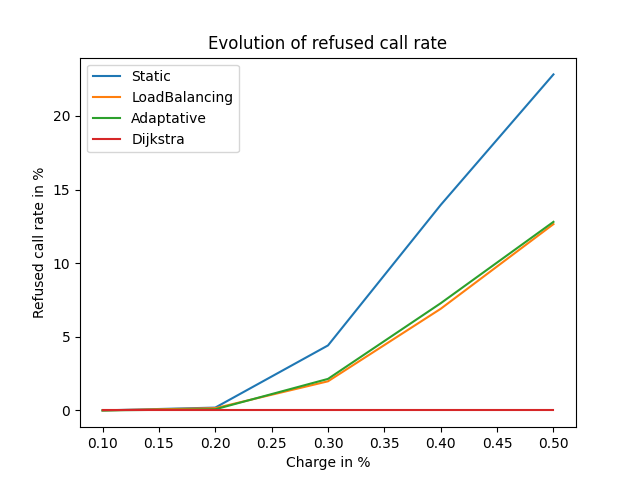
\includegraphics[width=0.48\textwidth]{call_rate.png}
% coeff moyenne = 1000
% cts_wire = 50
% cts_ca_wire = 25
% cts_wire = 10
% user_count = 100
\end{center}
Please note that those results were obtained for 100 users equally partitioned between the CAs. The
links wapacities were (50, 25, 10).\\
These results corresponded our expectations as the Static method's performance quickly deteriorated with the network load. Indeed, 
this method is not able to avoid filling in the already overencumbered links of the network.\\
To furthermore elaborate our comparison of the algorithms, we decided to simulate network failures in different ways:
\begin{enumerate}
        \item The first way of simulating a failure was by creating ``link'' failures by artificially filling them up. We tried to fill
        20\% of the links pior to simulation. These were the obtained results:
        \begin{center}
                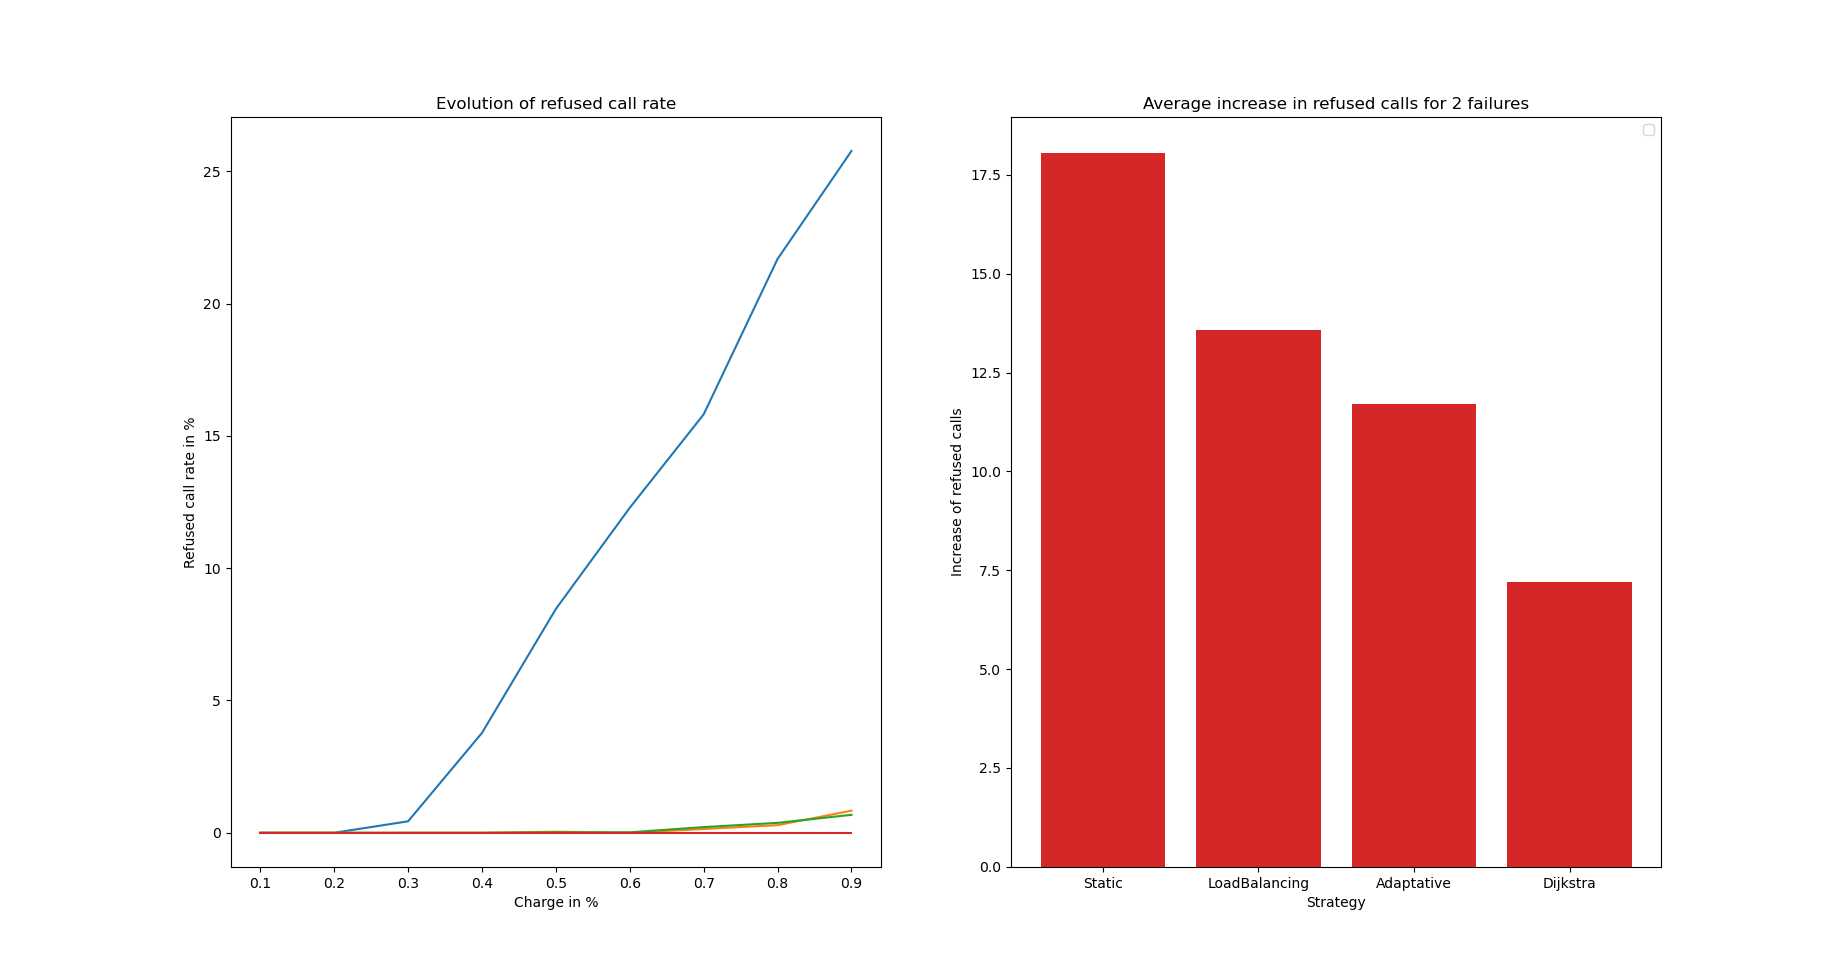
\includegraphics[width=0.48\textwidth]{link_failures.png}       
        \end{center}
        This result could have been predicted, as the more dynamic routing algorithms still are the most resilient to that kind of failure.
        \item The second way of simulating a failure was this time by imitating a node failure, which would then be the equivalent of a 
        switch failure. To do so, firstly slightly increased the size of the network to allow more possibility for the selected routes:
        we went from 2 CTS, 3 CA to 4 CTS, 5 CA.Then, we randomly elected switches of the network and artificially filled all the links
        connected to it. That way, it was impossible for a communication to go through that switch. These were the obtained results:
        \begin{center}
                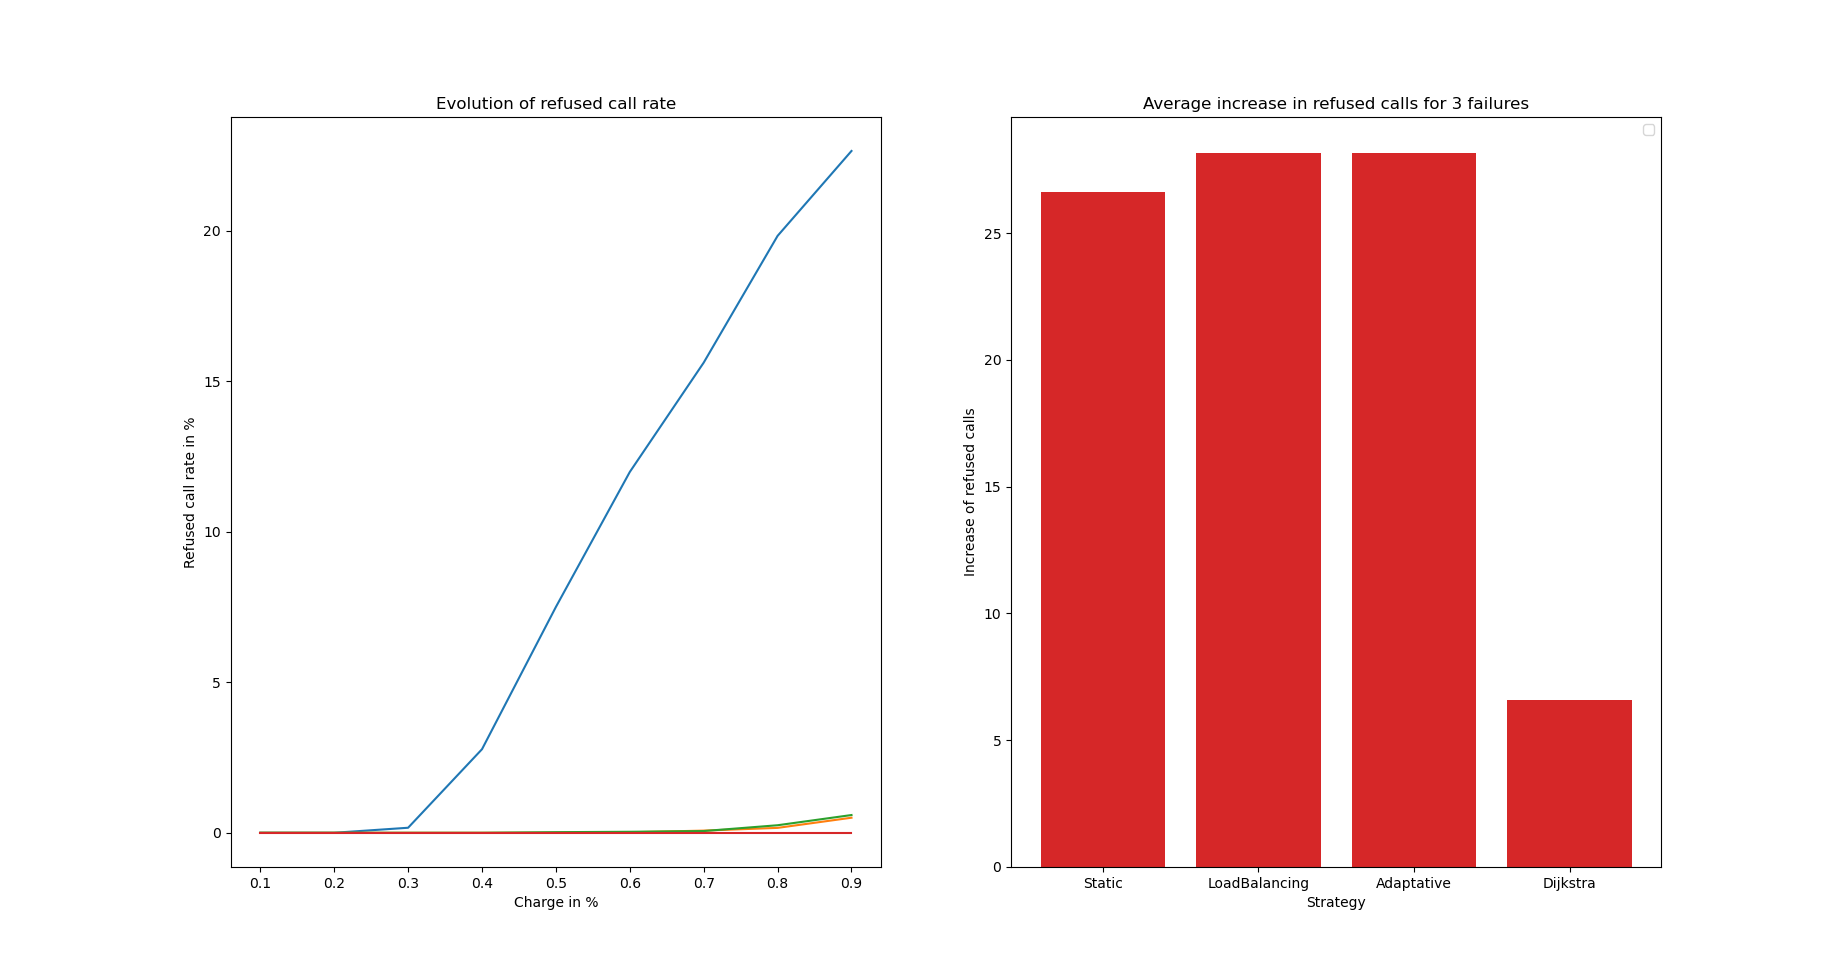
\includegraphics[width=0.48\textwidth]{node_failures.png}       
        \end{center}
        Here, we can see that nodes failures tend to affect more heavily the routing algorithms than the previous simulation. Even though
        this is partially due to the fact that incidentally, more links had to be filled in order to simulate that failure than the previous
        one, an interesting trend can be observed. As it could have been mathematically proven using the different algorithms, the modified
        Dijkstra algorithm is more often able to find a road thanks to its way of representing full links (the inversion of the matrix creates
        +Inf cells that are automatically ignored by the routing algorithm).
        \item A third way we tried altering the network was by simply ``deleting'' the link by putting its capacity value to 0. The problem in
        that way of doing was that the different algorithms are mostly based on scouting the currently active communications going through
        the commutator, hence the idea of our modified Dijkstra algorithm. Because the results did not provide an insightful result, we chose
        not to show them.\\
        Using our source code, this result can still be obtained by using the appropriate $``generer\_pannes\_X''$ function.
\end{enumerate}
\subsection{At a bigger scale}
One might wonder what would happen if we were to increase the size of the experiment. We decided to do so by running a new set of tests after
having increased all the different variables of the test.
It is important to note that the following tests are being performed with the first type of failures being present, being link failures.\\
We will associate the folliwing variables to each test: (\textbf{CTS count}, \textbf{CA count}, \textbf{Client count}).
\begin{itemize}
        \item Reference: the tests performed in the previous network had around (\textbf{3}, \textbf{4}, \textbf{100}) as an average.
        \item For (\textbf{12}, \textbf{13}, \textbf{800}), even though many more clients were going to use the network,
        we decided to only double the different link capacities. Here are the results:
        \begin{center}
                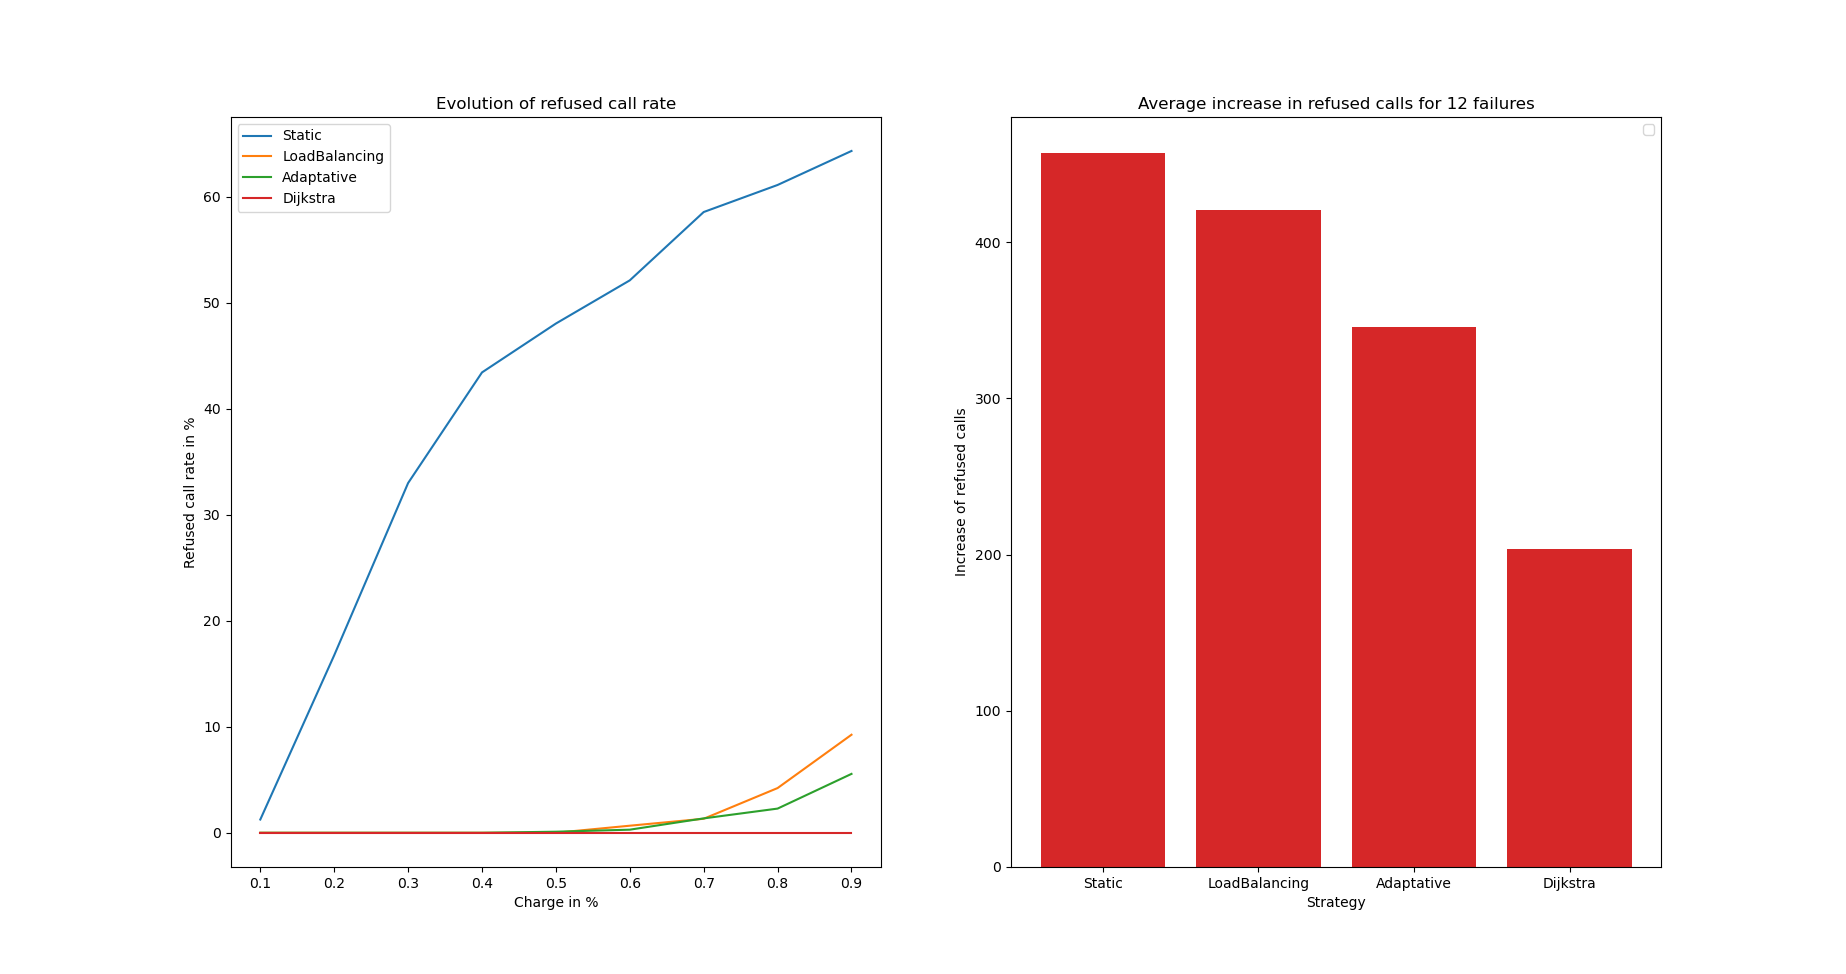
\includegraphics[width=0.48\textwidth]{bigger_network.png}       
        \end{center}
        As expected, the refused call rate on the left has significantly increased due to the increase of simultaneous users for a small
        increase of the link capacities. This showcases the scalability of our modelization. On a side note, we can notice that adding
        a same percentage of link failures (20\%) in a larger network produces the same result in terms of comparative increase of refused calls
        between the different algorithms. 
        \item Due to the duration of the execution of tests at a bigger scale, we came back to a network of a more reasonable size
        (\textbf{5}, \textbf{6}, \textbf{200}), but we decided to customize the links capacities.
        \begin{itemize}
                \item Without links between CA [inter CTS capacity: 30, CTS-CA capacity: 15, inter CA capacity: 0], we get the following result:
                \begin{center}
                        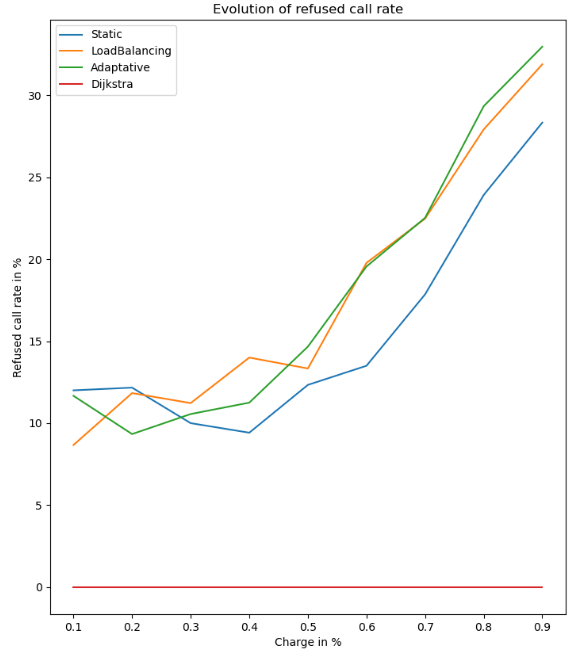
\includegraphics[scale=0.30]{without_CA_links_1.png}   
                        %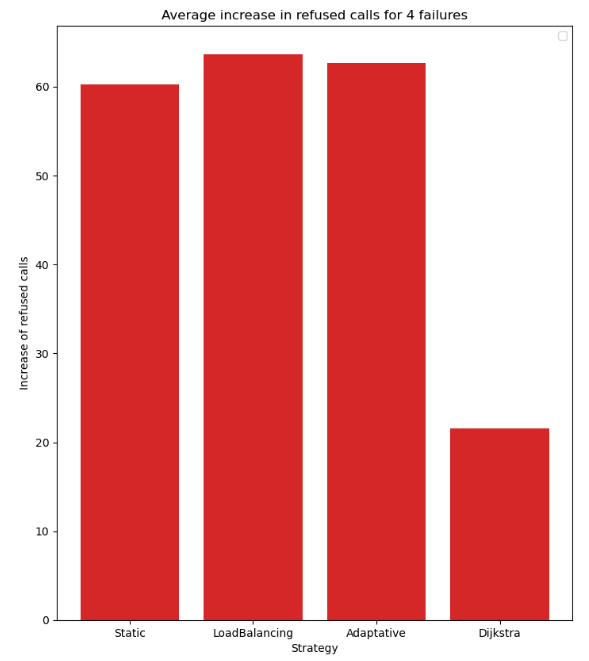
\includegraphics[scale=0.30]{without_CA_links_2.png} % jsp si cest bien utile    
                \end{center}
                which showcases the importance of side links in the network for a routing algorithm to be effective. In our case, the absence
                of CA-CA links removed a lot of possibilities for the routing algorithms, explaining the similarity in performance of the three
                main algorithms. On the other hand, Dijkstra's algorithm being able to choose a longer path to get to destination allows it to
                always find a route when no failure is in the network.
                \item With all links having the same initial capacity [all links: 15], we notice an evolution in the rate of refused calls for
                all the algorithms.
                \begin{center}
                        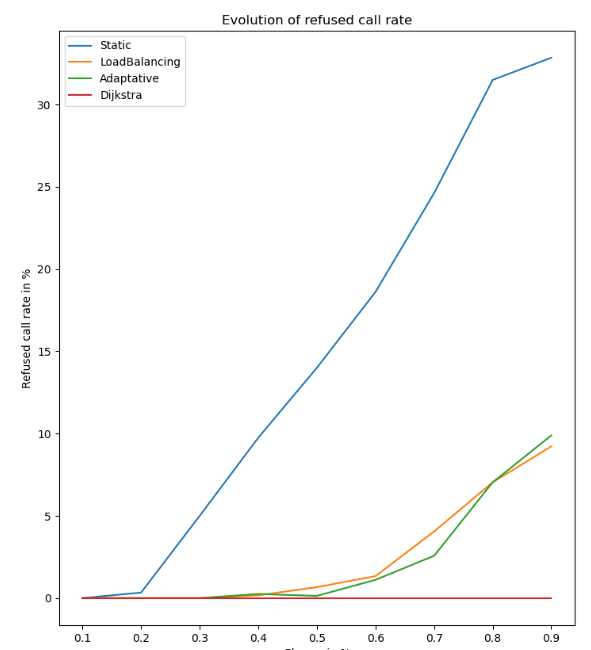
\includegraphics[scale=0.30]{same_capacities_1.png}
                        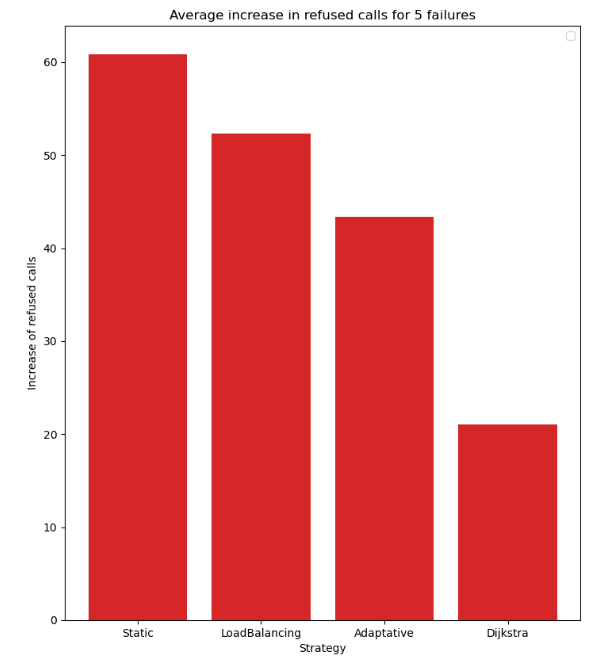
\includegraphics[scale=0.30]{same_capacities_2.png}
                \end{center}
                This is due to the fact that on one hand, the static method has comparatively better results thanks to the random choice of the
                communication source and destination, and on the other hand the repartition done by the load balancing and adaptative algorithms
                cannot use the capacity as a deciding factor anymore.
        \end{itemize}
\end{itemize}
\section{Bibliography}
\begin{itemize}
        \item BEYLOT, A.-L. (2022). PSTN networks courses for Enseeiht. 
        \item Scipy. (n.d.). The Dijkstra algorithm - Scipy . scipy.sparse.csgraph.dijkstra.
        Retrieved from https://docs.scipy.org
\end{itemize}
\end{document}


